
\begin{figure}[h]
    \centering
    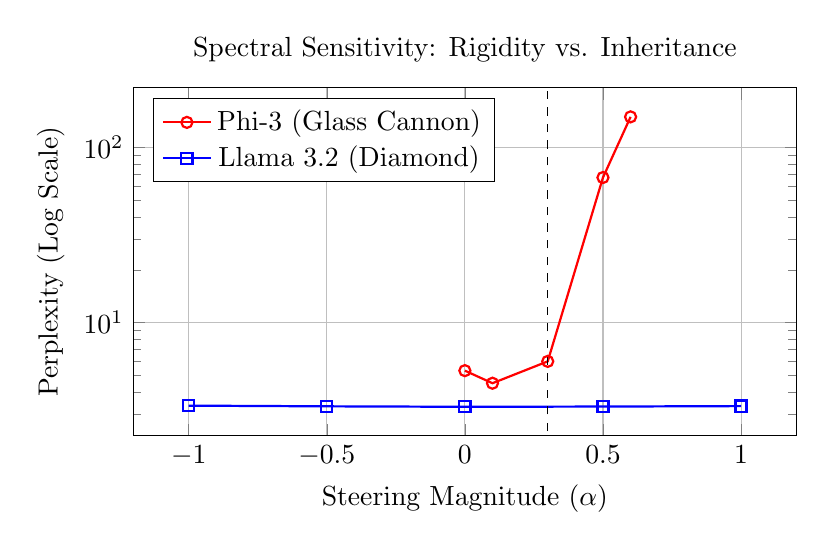
\begin{tikzpicture}
        \begin{semilogyaxis}[
            title={Spectral Sensitivity: Rigidity vs. Inheritance},
            xlabel={Steering Magnitude ($\alpha$)},
            ylabel={Perplexity (Log Scale)},
            grid=major,
            legend pos=north west,
            width=10cm, height=6cm
        ]
        
        % Phi-3
        \addplot[color=red, mark=o, thick] coordinates {
            (0.0, 5.31) (0.1, 4.5) (0.3, 6.0) (0.5, 67.5) (0.6, 150.0)
        };
        \addlegendentry{Phi-3 (Glass Cannon)}
        
        % Llama 3.2
        \addplot[color=blue, mark=square, thick] coordinates {
            (-1.0, 3.35) (-0.5, 3.32) (0.0, 3.30) (0.5, 3.31) (1.0, 3.33)
        };
        \addlegendentry{Llama 3.2 (Diamond)}
        
        \draw [dashed, black] (axis cs:0.3, 1) -- (axis cs:0.3, 1000);
        
        \end{semilogyaxis}
    \end{tikzpicture}
    \caption{The 'Diamond vs. Glass' topology. Llama 3.2 is spectrally invariant (flat PPL), while Phi-3 is extremely sensitive, validating the 'Inheritance' theory.}
    \label{fig:sensitivity}
\end{figure}
